
\section{Appendix}


\textbf{Q}: A query string (a string for which one wishes to determine the probability of).

\textbf{bestE}: A map from indices i of Q to the optimal encoding of Q[:i].

\textbf{minE}: A map from indices i of Q to $|bestE[i]|$

\textbf{opEnd}: A map from indices i of Q to the set of strings in $\Sigma'$: $\{x \in \Sigma' s.t Q[i-|x|:i] == x\}$


\begin{figure}[ht!]
\centering

\includegraphics[width=60mm]{uCOREPICS/DL/doubleLoopImage.png}
\caption{Double Loop Environment\label{overflow}}
\end{figure}

\begin{figure}[ht!]
\centering
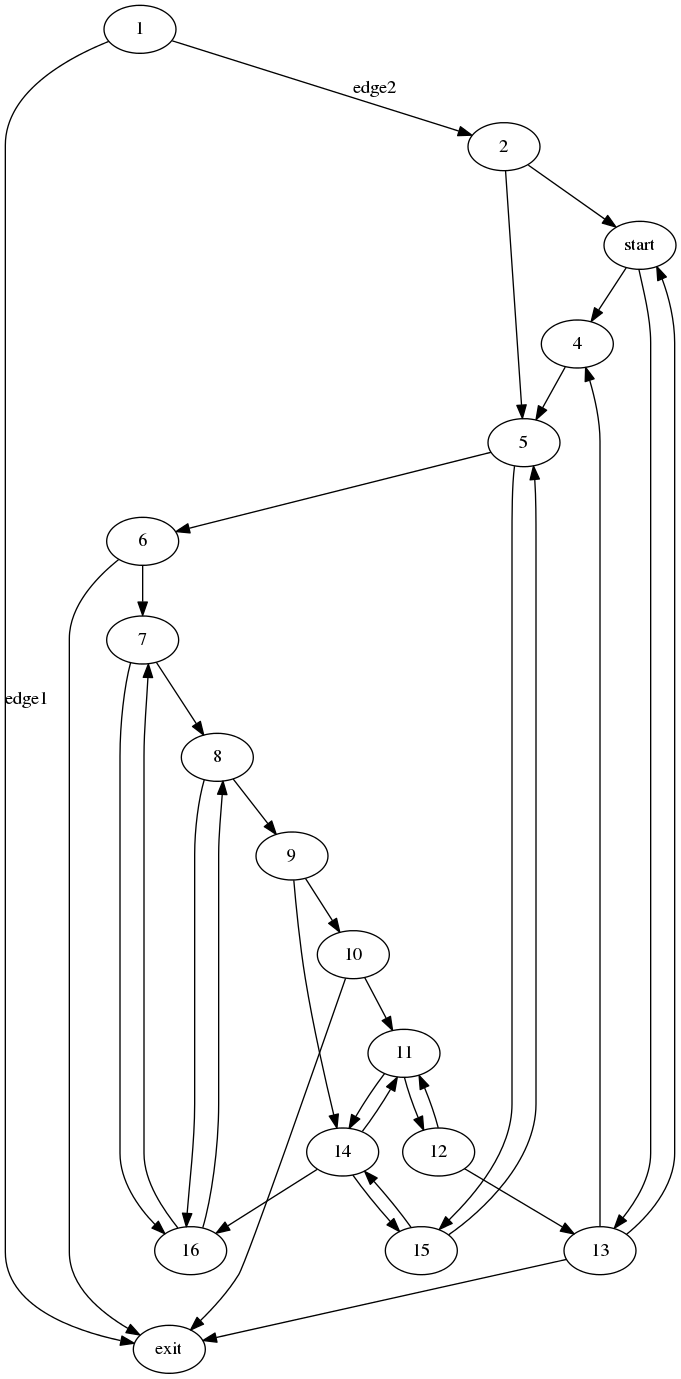
\includegraphics[width=40mm,height=60mm]{uCOREPICS/Pacman/graphPacMan.png}
\caption{Graph of Pacman Labyrinth\label{overflow}}
\end{figure}

\begin{algorithm}
\caption{Base Selection Algorithm}
\label{Base Selection}
\begin{algorithmic}[1]
\Procedure{Base Selection}{}
\State $\Sigma' \gets \{s, s \in \sum \}$
\State $Subs \gets \{$k frequent $s \in subObs\}$

\State $prevBestE \gets null$
\For{each obs in Obs}
	\State $prevBestEncoding[obs] \gets |obs|$
\EndFor

\State $i \gets 0$\
\While{$i<numOperators$}
	\State $bestOp \gets null$
	\State $bestImp \gets null$
	\For{each s $\in Subs$ }
		\State $c \gets 0$
		\For{each obs in Obs}
			\State $c \gets c+DPEncode(obs)-prevBestE(obs)$
		\EndFor
		
		\If{$c>bestImp$}
			\State $bestOp \gets observation$
			\State $bestImp \gets c$
		\EndIf
		
	\EndFor

	\State $\Sigma' \gets \Sigma' \cup bestOp$
	\For{each obs in Obs}
		\State $prevBestE \gets DPEncode(obs,\Sigma'$) 
	\EndFor	
	
	\State $i \gets i + 1$
\EndWhile 
\State \Return $\Sigma'$

\EndProcedure
\end{algorithmic}
\end{algorithm}

\begin{algorithm}
\caption{Encoding Algorithm}
\label{Encoding Algorithm}
\begin{algorithmic}[1]
\Procedure{DPEncode}{}

\State $bestE[] \gets String[|Q|+1]$
\State $minE[] \gets Int[|Q|+1]$
\State $opEnd[] \gets String[|Q|+1][]$

\State $bestEnd[0] = Q[0]$
\State $minE[0] = 0$

\For{i in $[1,|Q|]$}
	 \State $opEnd[i] \gets \{s \in \Sigma', Q[i-|s|:i] == s\}$
\EndFor

\For{i in $[1,|Q|]$}
	\State $bestOp \gets null$
	\State $m \gets null$ 
	\For{$s \in opEnd[i]$}
		\State $tempInt \gets minE[i-|s|] + 1$
		\If{$m == null$ or $tempInt < m$}
			\State $m \gets temp$ 
			\State $bestOp \gets s$
		\EndIf
	\EndFor
	\State $minE[i+1] \gets m$
	\State $bestE[i+1] \gets bestE[i-|bestOp|] + bestOp$
\EndFor

\State \Return $bestE[|Q|]$

\EndProcedure
\end{algorithmic}
\end{algorithm}





